% Here is a suggested template for PhD research proposal for the
% first annual report.
% Written originally 2010-06-22 by T. W. Yee.
% Last modified      2010-07-22 by T. W. Yee.


\documentclass[12pt,a4paper]{article}


\usepackage{natbib}    % For BibTeX
\usepackage{graphicx}  % To import .pdf files
\usepackage{hyperref}

\hypersetup{
	linkcolor  = black,
	citecolor  = black,
	urlcolor   = blue,
	colorlinks = true
}

\usepackage{array}
\newcolumntype{L}{>{\raggedright\arraybackslash}m{5cm}}


 \oddsidemargin  -10mm
 \evensidemargin -10mm
 \headheight 0mm
 \headsep -3mm
\textheight 250mm
\textwidth 180mm
\topmargin -4mm
\topskip -10mm

%\textwidth=450pt
%\hoffset=-2cm


\begin{document}

\begin{Large}
\begin{center}
\textbf{COMPSCI 380 Project} \\
\textbf{Efficient mapping of spatial equity using R and OpenStreetMap} \\
\end{center}
\end{Large}

\begin{center}
\today \\
Christopher Vroegop \\
Student ID: 752236739 \\
cvro467@aucklanduni.ac.nz \\
\emph{The University of Auckland} \\
Supervisor: Dr Kaiqi Zhao
\end{center}



% ----------------------------------------------------------------------
\section{Abstract}
\label{sec:abstract}

Spatial equity concerns the equity of the spatial distribution of amenities. Analysis and visualisation of spatial equity has traditionally been a slow process requiring substantial data cleaning and merging. This report outlines a novel framework through which OpenStreetMap and R can be used to quickly perform spatial equity analysis across large areas. It implements two algorithms to do so -- density of amenities and nearest neighbour. Both are implemented efficiently to enable millions of records to be processed quickly. Finally, the technique is applied to New Zealand data as a demonstration.

% ----------------------------------------------------------------------
\section{Introduction and background}
\label{sec:intro}


Spatial equity studies the spread of amenities and disamenities across an area, and asks whether it is fair. \cite{talen:2011} notes that ``geovisualization of spatial equity is of key importance because it communicates a fundamental concept [...]: who has access to things and who does not.'' Society is becoming every-more conscious of addressing past and present inequities, and spatial equity provides a framework to analyse this in a quantitative manner.

Two New Zealand examples of spatial equity studies include \cite{beere:2017}, who analysed the relationship between greenspace and academic achievement, and \cite{sushil:2017} who investigated New Zealand food swamps, areas where healthy food was hard to come by. 

However, both of these papers also demonstrate one of the fundamental challenges of spatial equity analysis - data sourcing. \citeauthor{beere:2017} determined the location of green space by combining three separate government datasets, while \citeauthor{sushil:2017} found food outlets by aggregating 66 councils' worth of data and supplementing it with listings from a restaurant aggregator.

Such slow and complicated analyses are probably necessary to ensure high quality data. However, it makes the new discoveries in spatial equity analysis extremely slow - if a spatial equity researcher wishes to study a new area of interest, they must spend weeks compiling data before they even know if it contains anything of interest.

This report demonstrates a novel way of approximating spatial equity, using raster analysis in R and data from OpenStreetMap to quickly and efficiently approximate equity statistics for millions of individual locations, and then aggregate them for display. Using this framework, researchers can rapidly analyse spatial equity across a wide range of amenities.

The framework is written using the GIS capabilities of the R programming language. This makes it flexible and highly extensible, and allows it to integrate well with other GIS software. It can be \href{https://github.com/Scienciser/spatialequityproject}{downloaded freely from GitHub}.

As a demonstration of the power of this framework, it was used to analyse New Zealand spatial equity for several amenities, including parks, fast food, supermarkets and schools, as described in Section~\ref{sec:demonstration}. This was then displayed on an \href{https://www.arcgis.com/apps/dashboards/2e46471d956347bcb0a1de8465ad31d7}{interactive website}.


% ----------------------------------------------------------------------
\section{Tools}
\label{sec:tools}

\subsection{OpenStreetMap}
\label{sec:osm}

OpenStreetMap \citep{osm:2021} is a crowd-sourced mapping website with more than seven million users that aims to create a comprehensive, free map of the world. It is widely used in the tech industry, providing much of the data for Apple Maps, as well as basemaps for Facebook and Snapchat, among many others. Its data is licenced under the Open Data Commons Open Database License, which allows it to be used freely by researchers provided that OSM is credited.

Despite being crowd-sourced, OSM data quality is broadly seen as close to or on par with commercial providers, including Google Maps (\citealt{ciepluch:2010} and \citealt{helbich:2012}). This makes it an excellent starting point for our analysis.

The full OpenStreetMap dataset is freely available, and can be downloaded in the OSM format (formatted XML) from several locations, including the \href{https://download.geofabrik.de/}{Geofabrik OpenStreetMap Extracts} service. OpenStreetMap stores all map elements as one of points, ways (either lines or polygons) or relations (relationships between objects). Each OSM object includes a tag describing it, as a key-value pair, for example \emph{amenity=restaurant} or \emph{highway=motorway} \citep{osm_cont:2021}. 

As a result, rough classes of amenities can be extracted relatively easily by filtering an OSM extract for key-value pairs. This framework uses Osmium, a fast, GPLv3-licenced C++ library and attached command-line tool to perform this filtering \citep{osmium:2021}.

\subsection{R}
\label{sec:r}

The R programming language \citep{r:2021} was used for scripting the framework, including wrapping calls to Osmium, performing further filtering and data cleaning, and crucially, performing spatial analysis and aggregation, thanks to its broad range of add-on packages. 

The \emph{sf} package \citep{sf:2018} was used for its spatial data structures and point/area spatial analysis tools. Its interface with the Geospatial Data Abstraction Library (GDAL) \citep{gdal:2021} was used to read in the OSM files output by Osmium, as well as Esri GDB/Shapefile files for other data sources. The \emph{tidyverse} packages \citep{tidyverse:2019} were used for data cleaning and wrangling. Raster object creation and analysis was handled by the \emph{raster} package \citep{raster:2021}, extended by the \emph{fasterize} package \citep{fasterize:2021} for faster rasterisation. Finally, the \emph{nabor} package, a wrapper for the \emph{libnabo} C++ library \citep{libnabo:2012} was used for fast  k-nearest-neighbour calculations.

\subsection{Esri ArcGIS}

The project was intended to be free to maximise accessibility, and hence the use of proprietary software was minimised. All of the data processing and aggregation was performed using freely available R libraries. However, the Esri ArcGIS suite \citep{esri:2021} did see some use. ArcGIS Pro was used for visualisation and prototyping, and its R extension, \emph{arcgisbinding} was used for exporting ESRI Geodatabases. Users without Esri software can export to Shapefiles or GeoJSON instead, though these restrict layers to one per file, and Shapefiles in particular face restrictions on attribute name length.

Finally, ArcGIS Online and ArcGIS Dashboards were used to produce the \href{https://www.arcgis.com/apps/dashboards/2e46471d956347bcb0a1de8465ad31d7}{demonstration website}. These tools allowed a quick, low-code way to display spatial data online. Though a site could have been built manually in JavaScript using libraries like Leaflet, and then self-hosted, the focus of this project was building a data processing framework, and building a site would have slowed this down substantially. However, the framework remains platform-agnostic, and thus can be used to output spatial data for use in almost any front-end spatial visualisation.

\section{Methodology}
\label{sec:methodology}

\subsection{Types of data}
\label{sec:types}

The ``spatial'' in spatial equity means that quantifying it is inextricably linked to distance and area. This framework uses the following definitions for data:
\begin{itemize}
	\item \emph{Amenity points} -- the locations, as points (projected x-y coordinates) of amenities or disamenities. Points would be used for locations that are relatively small in relation to a neighbourhood. For example, NZ spatial equity analysis of supermarkets would use a feature layer of points corresponding to every supermarket in New Zealand.
	
	\item \emph{Amenity areas} -- the areas, as polygons of amenities or disamenities. Areas would be used for locations that are relatively large in relation to a neighbourhood. For example, NZ analysis of park accessibility would use a feature layer of every park in New Zealand.
	
	\item \emph{Addresses} -- in areas with good data, the locations of street addresses provide an excellent indication of population distribution across the area. This could be substituted with high-resolution population data; for example the NZ Census includes population data in 100-200 person blocks. In areas with poor data, the locations of settlements could be used as an approximation.
	
	\item \emph{Aggregation blocks} -- areas to aggregate results by. For example, in a city like Auckland, aggregating results by suburb makes visualisations more tangible and thus interpretable for viewers.
\end{itemize}

Though this work was performed in a New Zealand context, the framework produced is generic, and thus portable and applicable to anywhere with sufficient data quality.

\subsection{Amenity density vs nearest neighbour}

In measuring spatial equity, we are concerned with the \emph{accessibility} of amenities to individuals, for example, how easily can a person living in a specific location access a supermarket, or library, or school?

The obvious solution is \emph{amenity density} - the number, or area of amenities per unit area - for example, how many supermarkets are there in a suburb? 

\begin{figure}[!htbp]
	\begin{center}
		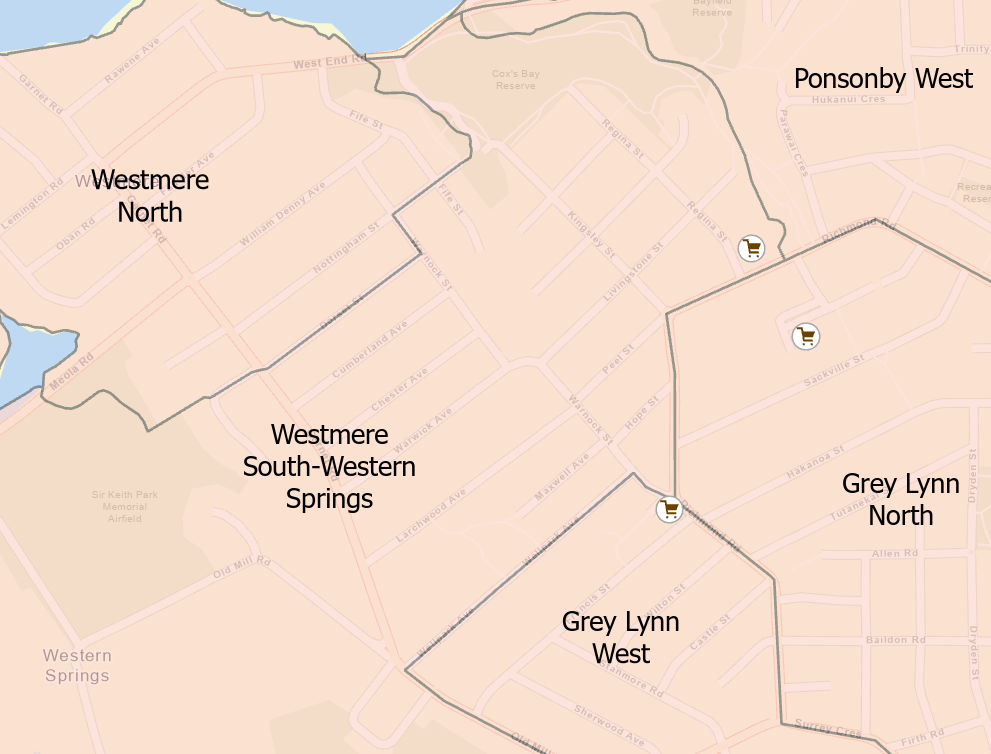
\includegraphics[height=100mm]{./figures/supermarkets_grey_lynn.PNG}
		\caption{Supermarkets and SA2 boundaries in Grey Lynn, Auckland, NZ}
		\label{fig:grey_lynn}
	\end{center}
\end{figure}

Figure~\ref{fig:grey_lynn} demonstrates the boundary issues created by such an approach, by showing an example of amenities clustered at the edges of aggregation blocks. Observe how the \emph{Ponsonby West} aggregation block does not contain any supermarkets itself, though in practice, residents there have are closer to supermarkets than those living in the west of \emph{Westmere South-Western Springs}. Adding a buffer around each aggregation block (as shown in Figure~\ref{fig:amenity_density}) would mitigate this at the expense of inaccuracy elsewhere, as now \emph{Westmere South-Western Springs} would be ``proximate to'' three supermarkets despite this only being true for residents at its eastern end.


\begin{figure}[!htbp]
	\begin{center}
		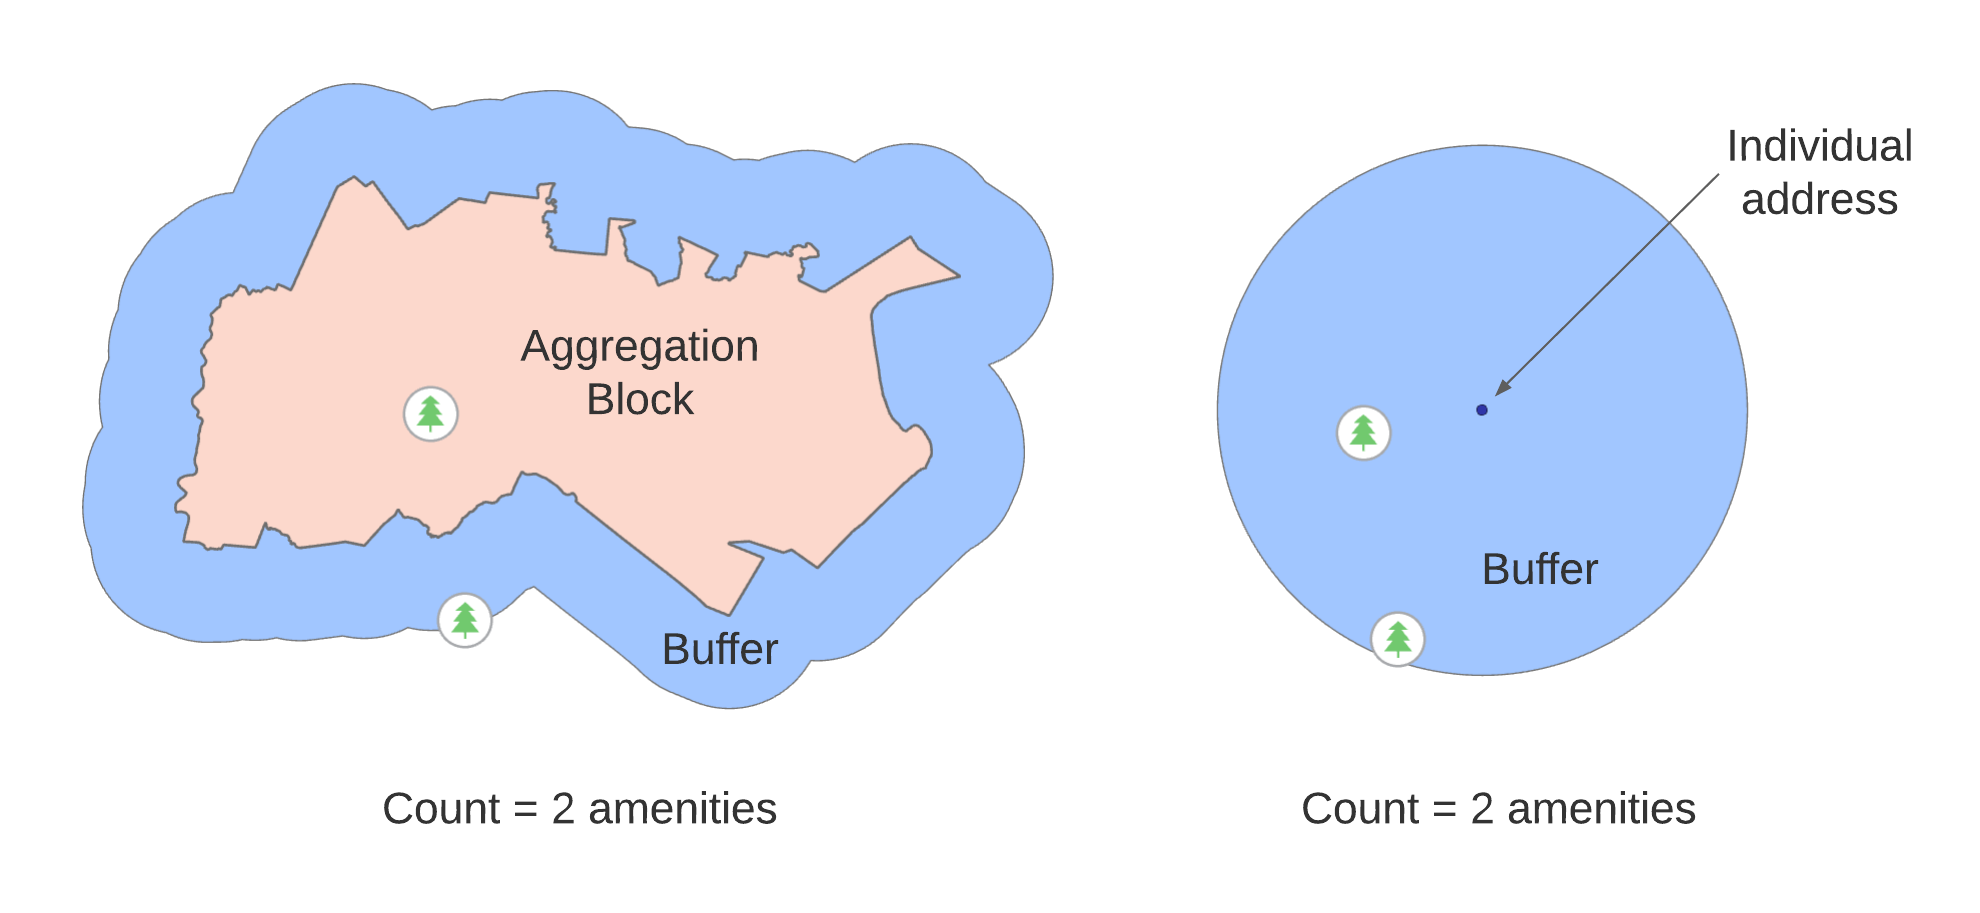
\includegraphics[height=80mm]{./figures/amenity_density.png}
		\caption{\centering Two types of amenity density calculations. On the left we count amenities by aggregation block, with a buffer to reduce boundary effects. On the right, we take the recommended approach of counting amenities by applying the buffer to each individual address. These results can then be aggregated across an aggregation block.}
		\label{fig:amenity_density}
	\end{center}
\end{figure}

This approach, but also other coarse-grained calculations of spatial equity across aggregation blocks run into a second issue - they implicitly assume uniform population density across each block. Figure~\ref{fig:tirau} demonstrates how addresses in some rural SA2 are concentrated in towns. Coarse analysis here could easily overestimate the accessibility of amenities for those in rural areas, as results from those in towns skew averages.

\begin{figure}[tt]
	\begin{center}
		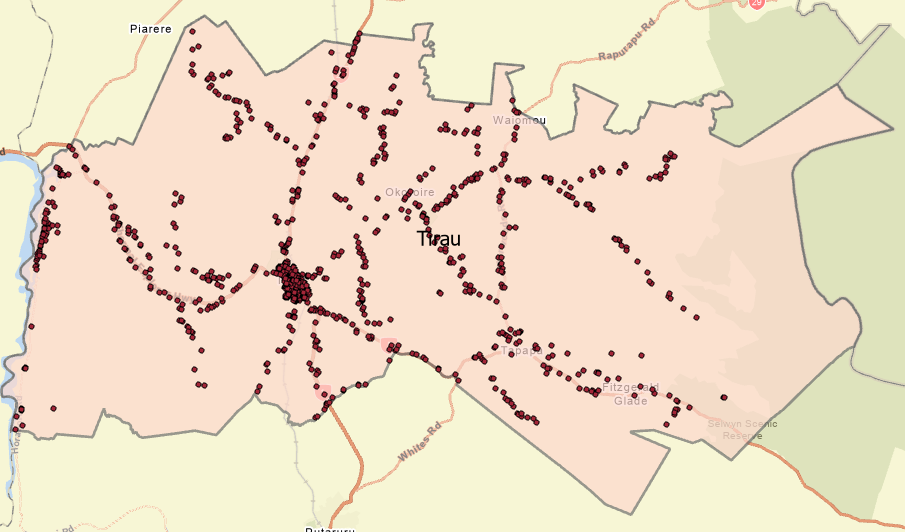
\includegraphics[height=80mm]{./figures/tirau.png}
		\caption{Street addresses in Tirau, NZ}
		\label{fig:tirau}
	\end{center}
\end{figure}


This second issue is best mitigated by performing amenity density calculations with very fine-grained blocks or even at a per-address level, as shown in Figure~\ref{fig:amenity_density}. This will ensure that the individual circumstances of each address are accounted for, though we still end up defining a hard cut-off past which we do not consider amenities. Furthermore, finer-grained calculation have an inevitable performance penalty, which must be balanced.

Not all amenities are created equal, and thus counting may not be the best metric. For example, an individual living within walking distance to three 500m\textsuperscript{2} parks arguably has access to worse amenity than an individual living within walking distance of one 50,000m\textsuperscript{2} park. However, amenity density allows us to weight amenities, for example by taking the sum of the area of park within an aggregation block.

An alternative approach is thus needed, we suggest \emph{nearest neighbour}. Here, the distance is calculated to the nearest instance of something - for example, how far is it for a resident to the nearest library, or the nearest supermarket?

Here, we lose information about the density of the amenity around an address - where amenity density will tell us how many supermarkets are close by, nearest neighbour will only tell us the distance to the nearest. However, we must ask, is being within walking distance to two supermarkets a substantial advantage over being within walking distance to just one? Consumers would gain more choice, and perhaps competition would bring prices down, but the marginal benefit is much less than that of the first. 

We also avoid the problem of defining hard borders - even the most remote locations will have a nearest neighbour, despite the density of amenities within the region being zero.

Furthermore, whereas in amenity density summaries, non-homogeneous amenities can be weighted, for example parks by area, under nearest neighbour, they cannot. Thus, users must take care that all amenities in such an analysis are comparable.

Once again, fine-grained or per-address nearest neighbour calculations produce better results. Taking Figure~\ref{fig:grey_lynn} as an example again, assigning all addresses in an aggregation block the distance from the centroid of that block to the nearest neighbour will yield substantial inaccuracy, particularly at the block's edges. However, once again, fine-grained analysis yields substantial performance cost.

\begin{table}[!htbp]
	\caption{Summary of differences between amenity density and nearest neighbour}
	\centering % Center-align table
	\ ~~~~ \\ % Space between caption and table
	\label{tab:differences}
	\renewcommand{\arraystretch}{1.5} % Increase row margins
	\begin{tabular}{|L|L|L|}
		\hline
		& \textbf{Amenity density} & \textbf{Nearest neighbour} \\
		\hline
		Method & Aggregate amenities in a given area. & Find the nearest instance of an amenity from a set of points. \\
		\hline
		Boundary problems & Significant - location of edges and size of buffers can alter results. Partially mitigated by aggregating fine-grained calculations. & None. \\
		\hline
		Allows non-homogeneous amenities to be weighted & Yes. & No. \\
		\hline
		Provides information about more than one amenity & Yes. & No. \\
		\hline
	\end{tabular}
\end{table}

Each spatial equity analysis technique has its place, so an analyst must choose the best option given the characteristics of the amenity in question.

\section{Implementation}

\begin{figure}[!htbp]
	\begin{center}
		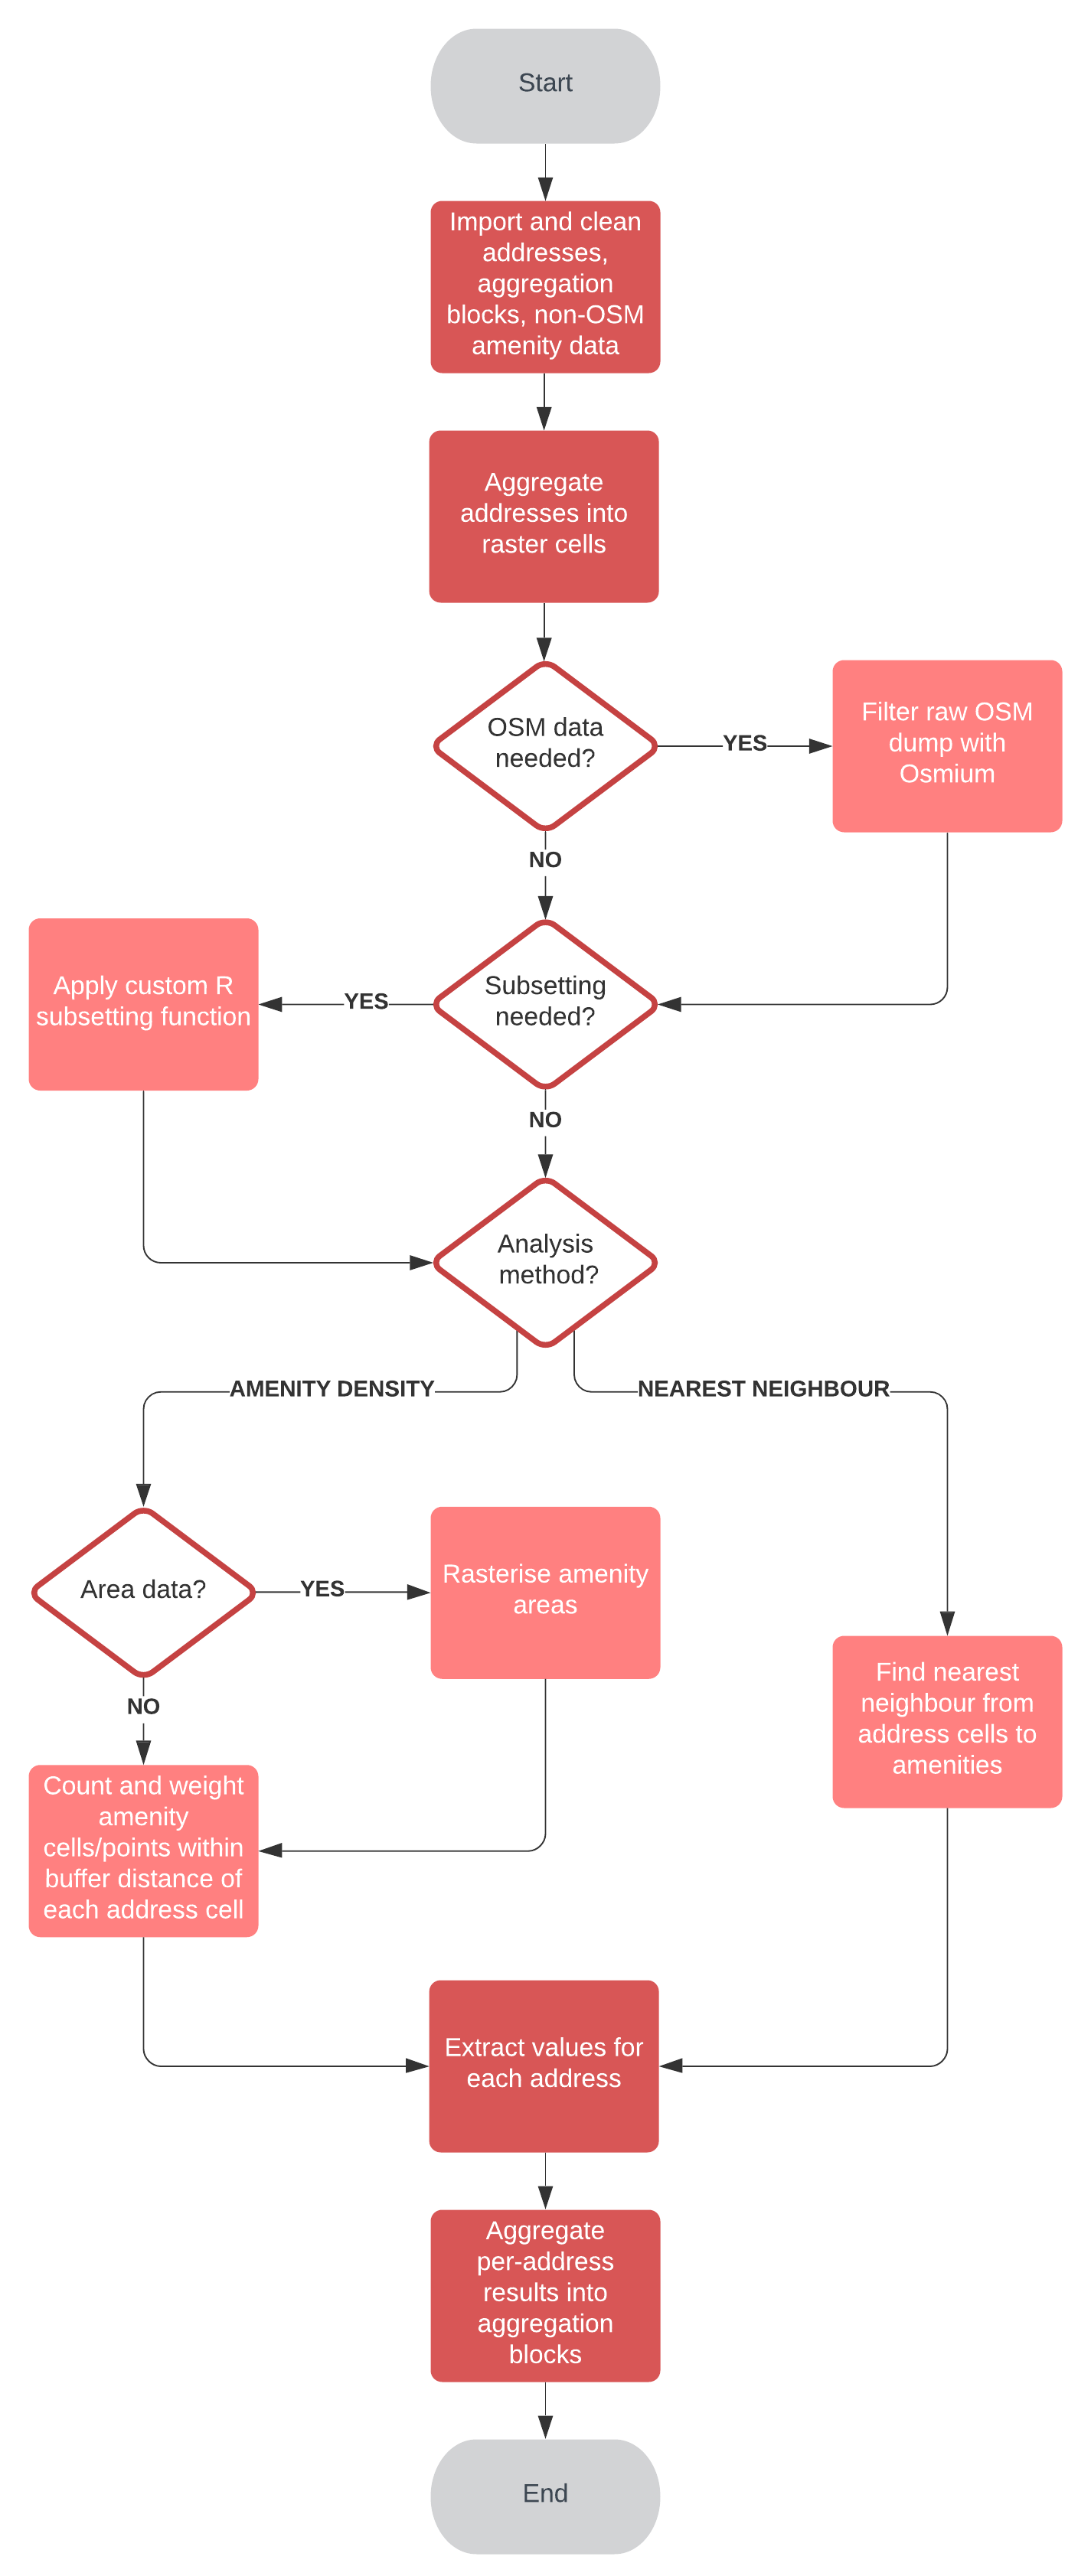
\includegraphics[height=220mm]{./figures/algorithm_flow.png}
		\caption{Program flow of spatial equity processing algorithm used.}
		\label{fig:flow}
	\end{center}
\end{figure}


This project implements an R library that allows for both amenity density and nearest neighbour analysis to be performed efficiently on arbitrary datasets, called \emph{spatialequityproject}. It can be \href{https://github.com/Scienciser/spatialequityproject}{downloaded freely from GitHub}.

A flowchart of the data processing pipline implemented is shown in Figure~\ref{fig:flow}.

First, the addresses and aggregation blocks (as described in Section~\ref{sec:types}) should be imported and cleaned, as well as projected to a global projected coordinate system of the user's choosing. Projection is crucial, since it allows calculations in fixed length units, like metres, rather than latitude and longitude coordinates. 

OpenStreetMap amenities data can be provided as an OSM dump, since the framework provides a wrapper for filtering it with Osmium; other amenities data needs to be sourced and cleaned manually.

Next, the addresses are processed. Given it was found that fine-grained analysis produced better results for both techniques, it was desirable to perform analysis on as close to individual addresses as possible.
However, this created performance issues - with an $n$ in the millions of addresses, even $O(n^2)$ algorithms became prohibitively slow.

The solution came from the observation that, at least in cities, most addresses are very close together. Apartment buildings have hundreds of addresses in almost identical locations, so analysing each individually results in significant redundant processing. A raster of 100m$\times$100m was fit (though this is user-customisable), and all addresses in each cell were assigned the coordinates of the cell's centre, with analyses being conducted once per cell. This results in a maximum error of $\sqrt{100^2+100^2}=141\textrm{m}$, which is easily low enough for even the most localised spatial equity analysis. This can be performed in $O(n)$ time and, in the case of New Zealand address data, results in one thirtieth the number of calculations required.

Next, if required, Osmium (see Section~\ref{sec:osm}) is used to quickly extract amenities from the OSM dump. If necessary, more fine-grained cleaning and subsetting can also be applied, with the library allowing custom R functions to be executed during the processing pipeline.

Then, the pipeline splits, depending on whether amenity density or nearest neighbour analysis is specified. 

\begin{figure}[tt]
	\begin{center}
		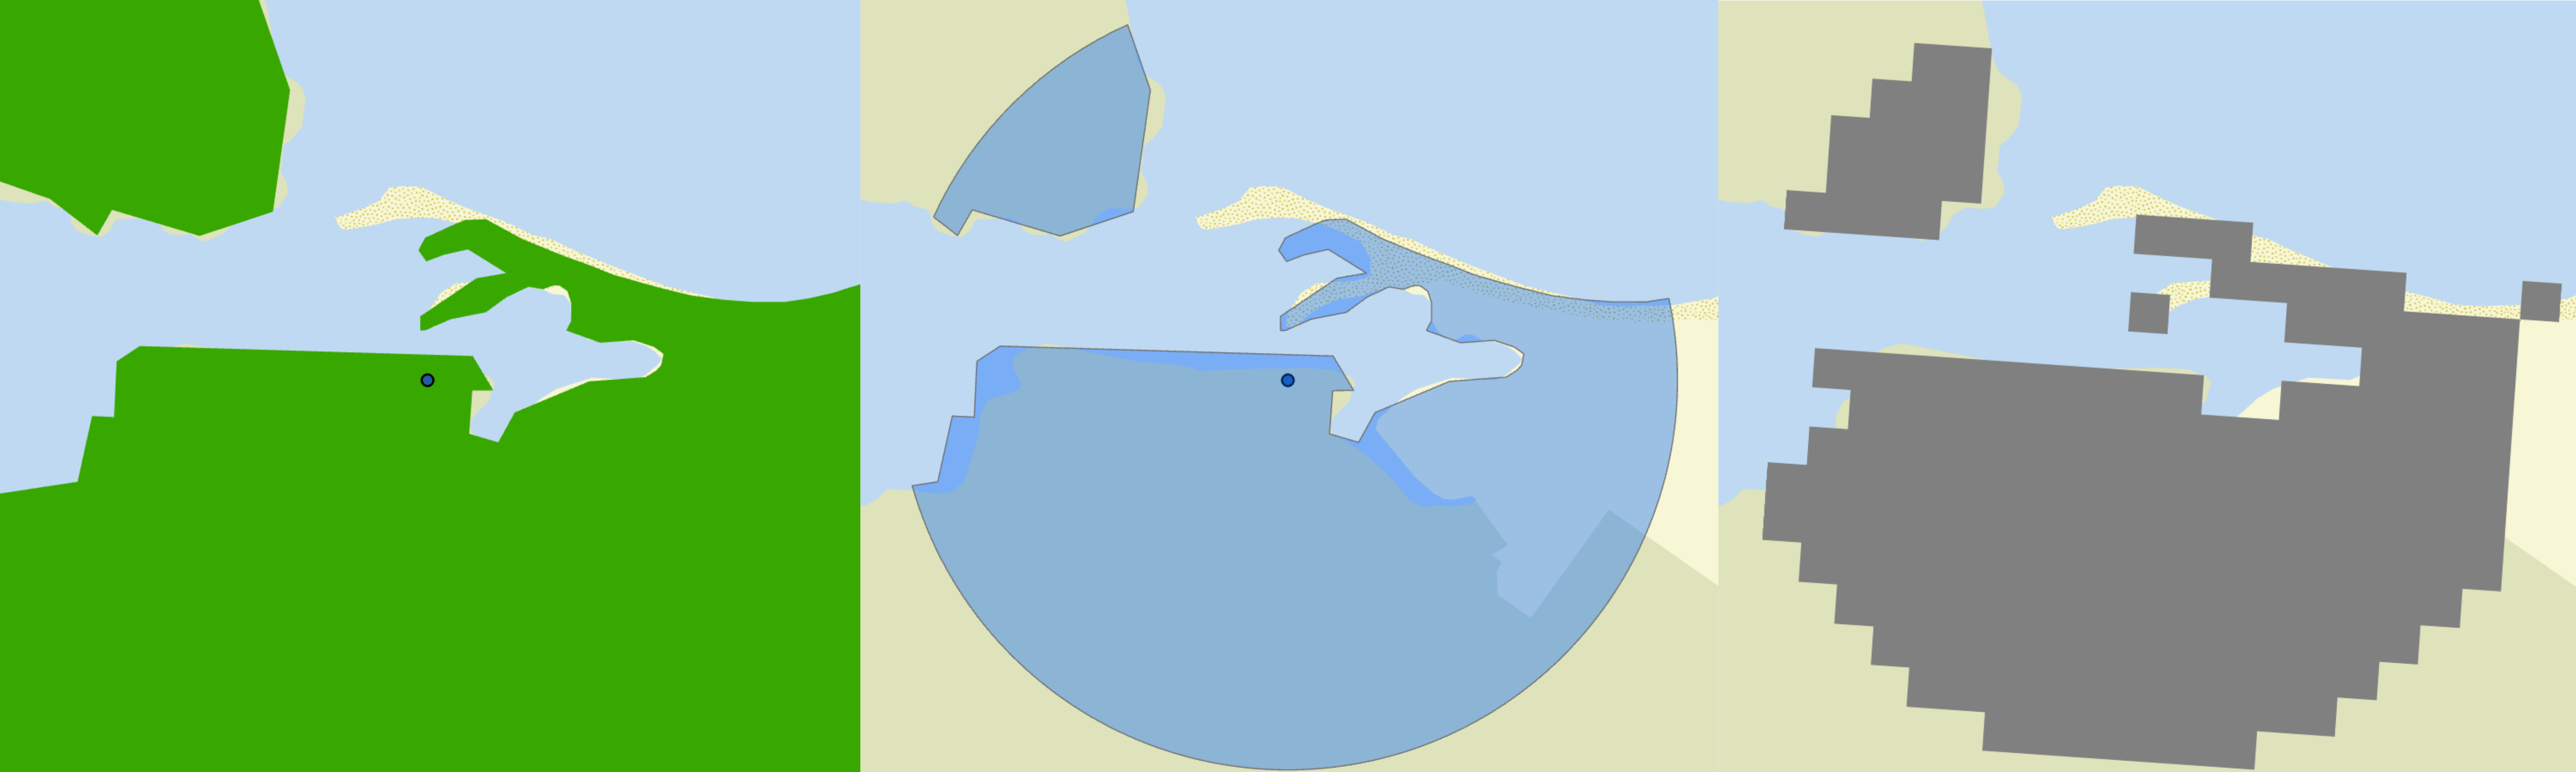
\includegraphics[width=180mm]{./figures/rasterisation.png}
		\caption{\centering Calculating amenity density for parkland through rasterisation. This is an extreme case in Abel Tasman National Park, where an address is almost entirely surrounded by national park (left). The goal is to quickly calculate the area of proximate parkland (centre), which is achieved by rasterising the parkland and then multiplying the number of cells in proximity to the address by their area (right).}
		\label{fig:raster}
	\end{center}
\end{figure}


Amenity density processing requires a set of points, so amenity area data is first rasterised to produce a set of amenity cells, allowing each polygon to be represented as a set of points given by the centroids of each cell. Then, for each address, the number of points within a buffer distance is counted. These can be weighted, for example in the case of parks, an address being proximate to three cells of area 100m $\times$ 100m is equivalent to being proximate to 30,000m\textsuperscript{2} of parkland. This process is demonstrated in Figure~\ref{fig:raster}. Given that for a fixed buffer distance, the maximum number of cells is fixed at $k$, this runs in $O(kn)$ time.

The nearest neighbour analysis was more straightforward. The method was implemented to only support amenity points, since the technique doesn't allow for weighting by area. As described in Section~\ref{sec:r}, the \emph{libnabo} nearest neighbour library was used \citep{libnabo:2012}, which provides an optimal k-nearest neighbours implementation in $O(n\log n)$ time. This finds the nearest amenity to each address cell, and gives the distance between them.

Finally, the results for each address are extracted from their corresponding address cell, and can be aggregated into aggregation blocks. The aggregation function is user-specified, though a median is recommended to avoid outliers skewing results. However, in rural aggregation blocks (e.g. Figure~\ref{fig:tirau}), this does risk high amenity access in regional towns obscuring the relative isolation of rural areas. Aggregation block selection is thus critical.


% ----------------------------------------------------------------------
\section{Demonstration}
\label{sec:demonstration}

In order to demonstrate the power of this framework, a demonstration was prepared. Its results are visualised on an \href{https://www.arcgis.com/apps/dashboards/2e46471d956347bcb0a1de8465ad31d7}{interactive ArcGIS dashboard}.

\subsection{Datasets used}
\label{sec:datasets}

The following sets of amenity points were used:

\begin{itemize}
	\item \emph{Libraries} -- OpenStreetMap extraction of tag \emph{amenity=library}. The data quality was deemed to be good; for instance all Auckland Council libraries plus university libraries were included.
	\item \emph{Major fast food outlets} -- OSM extraction of tag \emph{amenity=fast\_food} with entity name or brand fields containing \emph{McDonald's}, \emph{Burger King}, \emph{KFC}, \emph{Wendy's}, \emph{Pizza Hut} or \emph{Domino's}. The data quality was fairly good, though OSM coverage of outlets in shopping centre food courts was limited.
	\item \emph{McDonald's} -- subsetted from \emph{Major fast food outlets}.
	\item \emph{Supermarket chains} -- OSM extraction of tag \emph{shop=supermarket} with entity name or brand fields containing \emph{Countdown}, \emph{Pak'nSave}, \emph{New World}, \emph{FreshChoice}, \emph{Supervalue} or \emph{Four Square}.
	\item \emph{Countdown/New World/Pak'nSave} - large outlets subsetted from \emph{Supermarket chains}.
	\item \emph{Primary schools} -- a Ministry of Education dataset listing all schools in New Zealand with coordinates, subsetted by those offering tuition in at least Years 1-6.
	\item \emph{Intermediate schools} -- as above, but subsetted by those offering tuition in at least Years 7-8
	\item \emph{Secondary schools} -- as above, but subsetted by those offering tuition in at least Years 11-13.
\end{itemize}

The following set of amenity areas was used:
\begin{itemize}
	\item \emph{Parks} -- OpenStreetMap extraction of tags \emph{leisure=park,nature\_reserve} or \emph{boundary=protected\_area, national\_park}. The data quality was good - some parks were included that were unavailable in Google Maps data, though occasionally some areas were also missing.
\end{itemize}

The LINZ Data Service Street Address dataset was used to obtain all New Zealand street addresses \citep{linz:2019}. Analysis was performed across all 2.1 million addresses provided.

Stats NZ's Statistical Area 2 system was used for aggregration blocks, with each block containing approximately 1000-4000 people \citep{statsnz:2017}. These have the primary benefit of corresponding roughly to suburbs in cities and regions in rural areas, making choropleth maps produced with them highly interpretable.


\subsection{Results}

\begin{figure}[!htbp]
	\begin{center}
		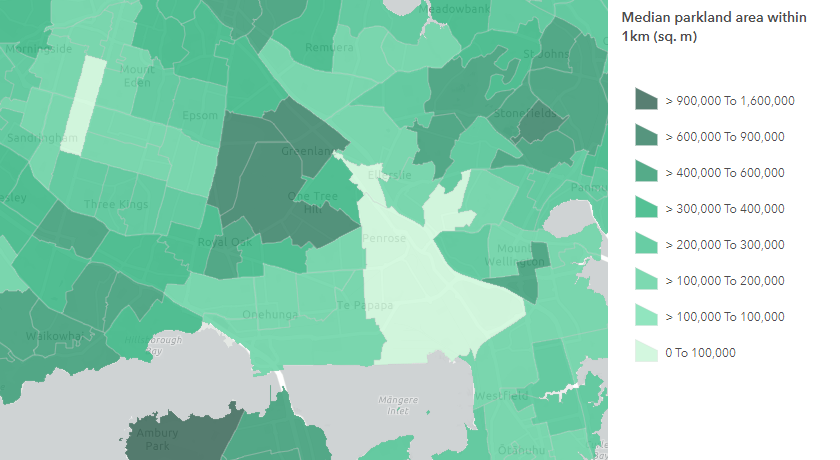
\includegraphics[width=170mm]{./figures/central_auckland_parks.png}
		\caption{\centering Auckland parkland coverage is generally good, though the industrial area in Penrose and those living in southern Mount Eden or Sandringham have less park access than most.}
		\label{fig:akl_parks}
	\end{center}
\end{figure}

\begin{figure}[!htbp]
	\begin{center}
		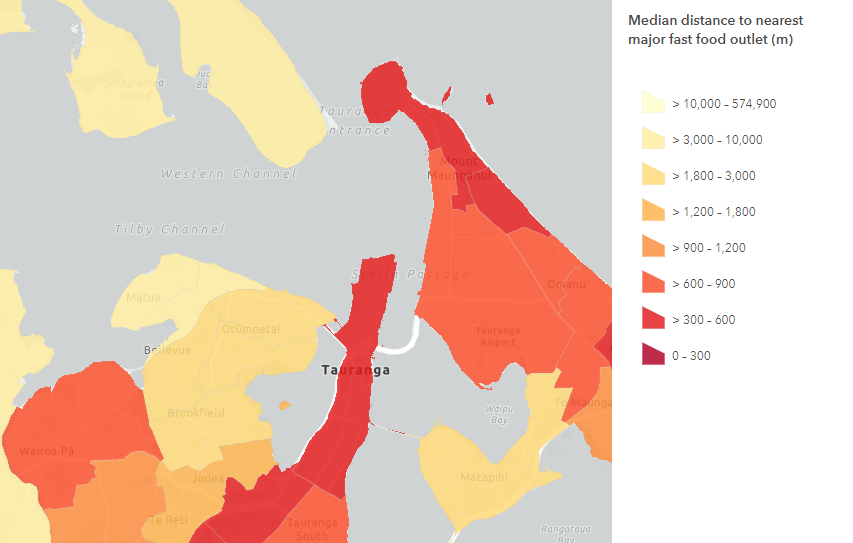
\includegraphics[width=170mm]{./figures/tauranga_fast_food.png}
		\caption{\centering While the CBD and Mount Maunganui are well covered, those looking for fast food in Tauranga's northeastern suburbs will be disappointed.}
		\label{fig:tauranga_ff}
	\end{center}
\end{figure}


\begin{figure}[!htbp]
	\begin{center}
		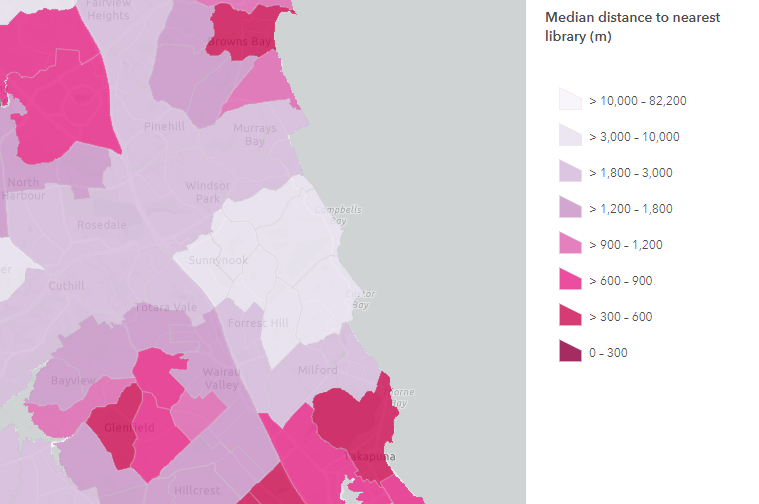
\includegraphics[height=100mm]{./figures/north_shore_libraries.png}
		\caption{\centering The Auckland library service fails to serve those in much of the eastern North Shore.}
		\label{fig:akl_libraries}
	\end{center}
\end{figure}

\begin{figure}[!htbp]
	\begin{center}
		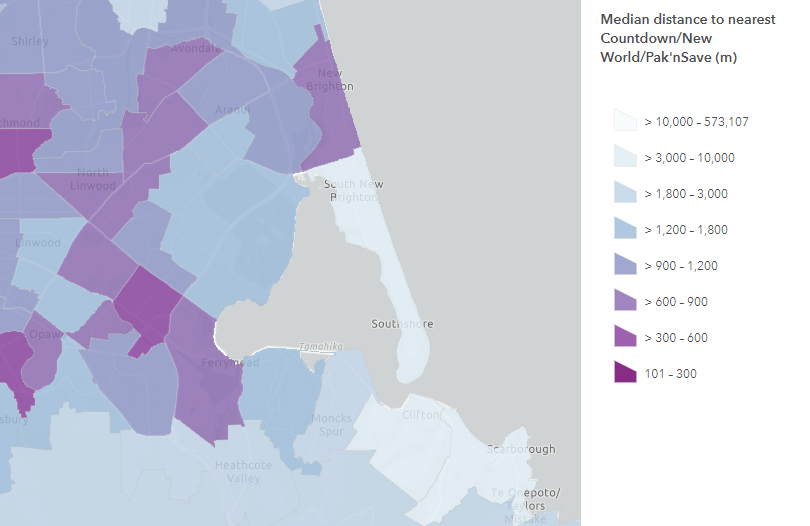
\includegraphics[height=100mm]{./figures/christchurch_supermarkets.png}
		\caption{\centering Christchurch's coastal suburbs, particularly Southshore, Redcliffs and Scarborough, are not served by major chain supermarkets.}
		\label{fig:chch_sm}
	\end{center}
\end{figure}

\begin{figure}[!htbp]
	\begin{center}
		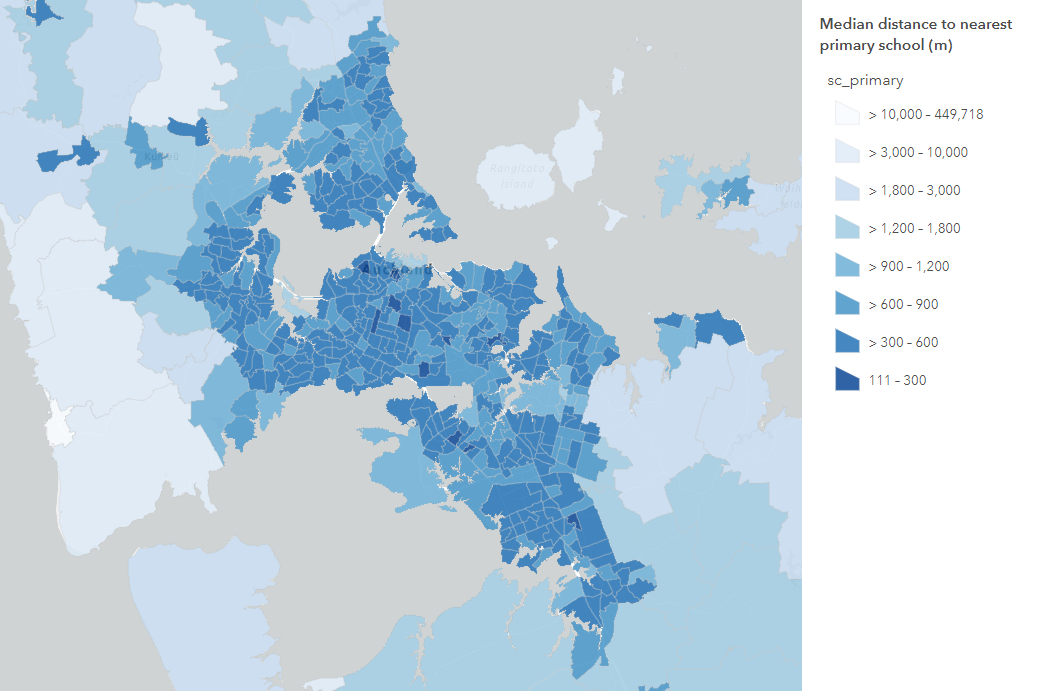
\includegraphics[height=100mm]{./figures/auckland_primary_schools.png}
		\caption{\centering Auckland is very well served by primary schools, with the median distance for almost every SA2 being less than 1200m.}
		\label{fig:akl_primschools}
	\end{center}
\end{figure}

Figure~\ref{fig:akl_parks} to Figure~\ref{fig:akl_primschools} provide a selection of insights on spatial equity in New Zealand that demonstrate the power of this framework. The processing time to produce all of these insights across every address in New Zealand was less than ten minutes, and the framework abstracts processing to such an extent that programming the analysis was also very quick. More detail on each of these results can be found on the \href{https://www.arcgis.com/apps/dashboards/2e46471d956347bcb0a1de8465ad31d7}{interactive dashboard}.

% ----------------------------------------------------------------------
\section{Conclusion}

In an increasingly urban society that is increasingly aware of its own shortcomings and inequities, being able to easily analyse and visualise spatial equity is increasingly important. This report has demonstrated a framework that allows just that - by leveraging the power of R and OpenStreetMap, insights can be gained quickly and efficiently. Where with traditional methods, analysis can take days of slowly piecing together datasets, this enables comparisons across a range of attributes in relatively little time.

There are plenty of opportunities to extend this work further. Other analysis techniques could be added beyond the two currently implemented, and the library could be made more generic, with the goal of publishing to CRAN. Visualisation techniques beyond choropleth maps could be explored to further mitigate boundary effects. 

However, as it is, this framework provides a strong jumping-off point for spatial equity analysis. By leveraging this, it is my hope that real inequities in our communities can be identified, and steps can be taken to mitigate them, creating a fairer society for all.

\addcontentsline{toc}{section}{References}
\bibliographystyle{elsarticle-harv} % Part of `elsarticle` package.

\bibliography{./myrefs}


\end{document}


